\documentclass{beamer}
\usepackage{tikz}
\usetikzlibrary{shapes.geometric, arrows.meta}

\title{LangChain and Document Retrieval with TypeSense and FAISS}
\author{Mostafa Razavi Ghods}
\date{\today}

% Define TikZ styles for blocks and arrows
\tikzstyle{startstop} = [rectangle, rounded corners, minimum width=3cm, minimum height=1cm,text centered, draw=black, fill=red!30]
\tikzstyle{process} = [rectangle, minimum width=3cm, minimum height=1cm, text centered, draw=black, fill=orange!30]
\tikzstyle{arrow} = [thick,->,>=stealth]

\begin{document}
	
	\frame{\titlepage}
	
	\begin{frame}
		\frametitle{What is LangChain?}
		\begin{itemize}
			\item LangChain is a framework for building applications powered by language models.
			\item It provides tools to manage and interact with language models effectively.
			\item LangChain simplifies the process of chaining multiple language model calls together.
		\end{itemize}
	\end{frame}
	
	\begin{frame}
		\frametitle{What are Chains in LangChain?}
		\begin{itemize}
			\item Chains are sequences of calls to language models or other computational steps.
			\begin{itemize}
				\item Example: First, a text summarization model processes the input text, and then a translation model translates the summary into another language.
			\end{itemize}
			\item They allow for complex workflows and tasks to be broken down into manageable steps.
			\begin{itemize}
				\item Example: An email filtering system might first classify emails into different categories and then summarize the content of each email based on its category.
			\end{itemize}
			\item Chains can include loops, conditionals, and parallel processing.
			\begin{itemize}
				\item Example: A loop can be used to iterate through a list of documents, applying sentiment analysis to each one. Conditional statements can be used to handle different types of documents differently. Parallel processing can speed up tasks by processing multiple documents simultaneously.
			\end{itemize}
		\end{itemize}
	\end{frame}
	
	\begin{frame}
		\frametitle{Integration of TypeSense with LangChain}
		LangChain integrates with TypeSense to leverage its capabilities as a vector store while offering additional functionalities compared to a standalone FAISS library. Here's how it works:
		\begin{itemize}
			\item \textbf{Vector Embeddings:} LangChain first generates vector embeddings for your documents. These embeddings are mathematical representations that capture the semantic meaning of the text. You can use pre-trained models or custom methods to create these embeddings.
			\item \textbf{TypeSense Integration:} LangChain interacts with TypeSense through a wrapper class or library specifically designed for this integration. This wrapper class simplifies communication between LangChain and the TypeSense API.
			\item \textbf{Indexing Documents:} The LangChain tool using TypeSense adds the documents and their corresponding vector embeddings to a TypeSense collection. This collection acts like a specialized database optimized for fast vector similarity search.
		\end{itemize}
	\end{frame}

	\begin{frame}
		\frametitle{Integration of TypeSense with LangChain}
	
		\begin{itemize}
			\item \textbf{User Query:} When a user submits a query, LangChain sends it to the tool utilizing TypeSense.
			\item \textbf{Vector Similarity Search:} TypeSense performs a vector similarity search within the collection. It compares the user query's vector embedding to the embeddings of all the documents and retrieves the documents with the most similar vectors.
			\item \textbf{Additional Filtering (Optional):} A key advantage of TypeSense is the ability to combine vector search with attribute-based filtering. LangChain can leverage this feature to allow users to filter the search results based on document attributes (e.g., author, date, category) in addition to vector similarity.
			\item \textbf{Returning Results:} Finally, LangChain receives the most relevant documents from TypeSense and returns them to the user.
		\end{itemize}
	\end{frame}
	
	\begin{frame}
		\frametitle{TypeSense Integration Workflow}
		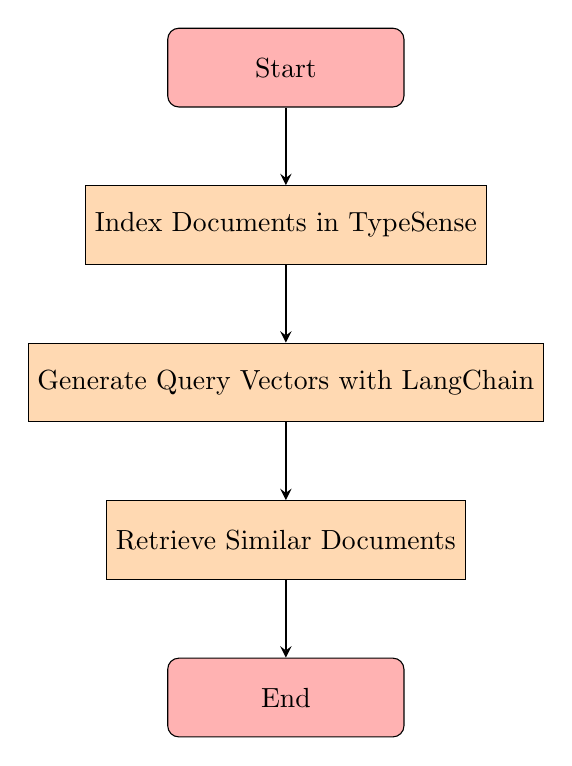
\begin{tikzpicture}[node distance=2cm]
			\node (start) [startstop] {Start};
			\node (index) [process, below of=start] {Index Documents in TypeSense};
			\node (query) [process, below of=index] {Generate Query Vectors with LangChain};
			\node (retrieve) [process, below of=query] {Retrieve Similar Documents};
			\node (end) [startstop, below of=retrieve] {End};
			
			\draw [arrow] (start) -- (index);
			\draw [arrow] (index) -- (query);
			\draw [arrow] (query) -- (retrieve);
			\draw [arrow] (retrieve) -- (end);
		\end{tikzpicture}
	\end{frame}
	
	\begin{frame}
		\frametitle{Benefits of Using TypeSense with Vector Stores in LangChain}
		\begin{itemize}
			\item \textbf{Faster Search:} TypeSense is optimized for fast in-memory search, making retrieval of similar documents efficient.
			\item \textbf{Richer Search Experience:} The ability to combine vector search with attribute filtering allows for more precise and user-friendly search experiences.
			\item \textbf{Easier Setup:} The LangChain integration with TypeSense simplifies the process compared to directly using FAISS.
		\end{itemize}
		In essence, LangChain uses TypeSense as a user-friendly wrapper around a vector store, enabling efficient vector similarity search with the added benefit of attribute-based filtering for a more comprehensive document retrieval experience.
	\end{frame}
	
	\begin{frame}
		\frametitle{Comparison: TypeSense vs FAISS}
		\begin{itemize}
			\item \textbf{TypeSense:}
			\begin{itemize}
				\item Designed for fast and relevant full-text search.
				\item Provides real-time updates and is easy to integrate.
				\item Better for small to medium-sized datasets.
			\end{itemize}
			\item \textbf{FAISS:}
			\begin{itemize}
				\item Developed by Facebook AI Research for efficient similarity search.
				\item Optimized for large-scale datasets.
				\item Supports various indexing methods for performance tuning.
			\end{itemize}
		\end{itemize}
	\end{frame}
	
	\begin{frame}
		\frametitle{Workflow with FAISS}
		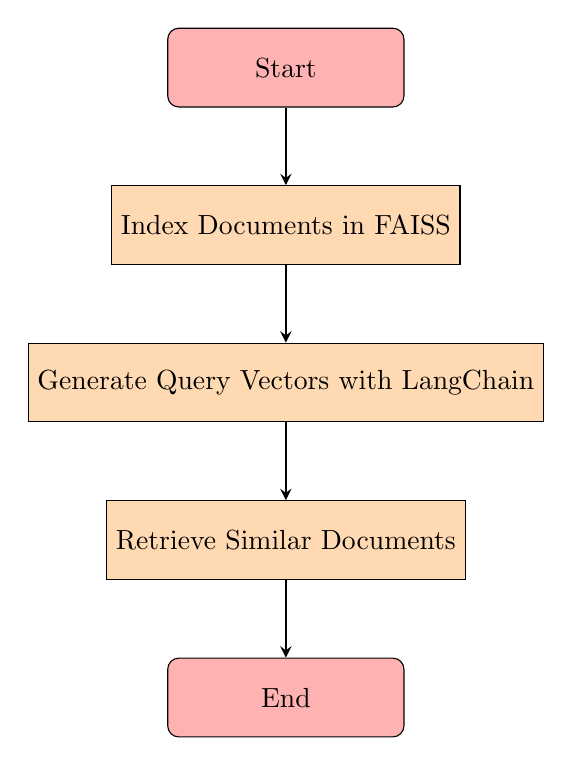
\begin{tikzpicture}[node distance=2cm]
			\node (start) [startstop] {Start};
			\node (index) [process, below of=start] {Index Documents in FAISS};
			\node (query) [process, below of=index] {Generate Query Vectors with LangChain};
			\node (retrieve) [process, below of=query] {Retrieve Similar Documents};
			\node (end) [startstop, below of=retrieve] {End};
			
			\draw [arrow] (start) -- (index);
			\draw [arrow] (index) -- (query);
			\draw [arrow] (query) -- (retrieve);
			\draw [arrow] (retrieve) -- (end);
		\end{tikzpicture}
	\end{frame}
	
	\begin{frame}
		\frametitle{TypeSense vs FAISS in Finding Similar Documents}
		\begin{itemize}
			\item \textbf{Performance:}
			\begin{itemize}
				\item TypeSense excels in real-time, full-text search.
				\item FAISS provides superior performance for large-scale vector searches.
			\end{itemize}
			\item \textbf{Ease of Use:}
			\begin{itemize}
				\item TypeSense is easier to set up and integrate for smaller projects.
				\item FAISS requires more configuration but offers more control for large datasets.
			\end{itemize}
			\item \textbf{Use Cases:}
			\begin{itemize}
				\item TypeSense is suitable for applications needing instant search with frequent updates.
				\item FAISS is ideal for applications dealing with extensive datasets requiring high retrieval speed.
			\end{itemize}
		\end{itemize}
	\end{frame}
	
	\begin{frame}
		\frametitle{Conclusion}
		\begin{itemize}
			\item Both TypeSense and FAISS are powerful tools for document retrieval.
			\item Choice depends on dataset size, real-time requirements, and ease of integration.
			\item LangChain provides a flexible framework to leverage these tools effectively.
		\end{itemize}
	\end{frame}
	
\end{document}
